\chapter{Modelando números $p$-ádicos}
\label{chapter2}


%Dado que el interés principal de este trabajo está enfocado al uso computacional de los números $p$-ádicos y dado que existen paquetes ofrecidos por \textit{Mathematica} para hacer cómputos aritméticos de números $p$-ádicos, encontramos que estos cómputos en general son puntuales, es decir, son operaciones número a número; Luego, la representación gráfica de los mismos queda en segundo plano. Además, la última fecha de revisión de los algoritmos es del año 1996; razón por la cual requerimos de una forma amigable y rápida de realizar estos cómputos, por lo tanto se hace necesario el uso de un lenguaje moderno y con nuevas estructuras de datos que permitan la eficiencia espacio-temporal\footnote{La eficiencia basada en el concepto de complejidad algorítmica.} de algoritmos sobre números $p$-ádicos.\\

%Usamos Python\footnote{Se requiere el uso de Python 3.5 en adelante.}, dado que es un lenguaje orientado a objetos y por ende permite un mejor diseño del cuerpo de números $p$-ádicos, además, permite representaciones simples de grafos y redes; más específicamente, nos basamos un paquete abierto ofrecido por la comunidad de desarrolladores, llamado %\textbf{NetworkX}\footnote{Para una documentación detallada acerca del paquete visitar: %\url{https://networkx.github.io/documentation/latest/_downloads/networkx_reference.pdf}}, dedicado a la creación, manipulación, estudio de estructuras, funciones y dinámica de redes complejas.

%\newpage

\section{La clase Número}
Como se mostramos en el capítulo \ref{chapter1}, la representación estándar de un número en $\Qp$ está dada por:
\begin{equation}
\sum_{k=-\infty}^{\infty} a_{k} p^{k}\text{, con $a_k\in\{0,\dots,p-1\}$ y $a_k=0$, para $k\leq - N$. 
}	\label{num_rep}
\end{equation}

Para modelar estas representaciones, se hace necesario restringirnos al caso de sumas finitas, luego, las principales características del número las representamos por medio de atributos y métodos.

\subsection{Diseño}
Definimos la clase Número     (\textit{number}) como sigue:


\begin{longtable}[c]{| c | c | c |}
	\caption{clase Número    (\textit{number}).\label{number_class}}\\
	
	\hline
	\multicolumn{3}{| c |}{Number}\\
	\hline
	\textbf{Atributo} & \textbf{Tipo} & \textbf{Descripción}\\
	$p$ & integer & Número primo\\
	$n$ & integer & Número entero negativo tal que ${p^n\leq \pnorm{x}}$\\
	$N$ & integer & Número entero positivo tal que ${\pnorm{x}\leq p^N}$\\
	%$m    (privado)$ & integer & Índice positivo donde la suma empezará\\
	%$M    (privado)$ & integer & Índice positivo donde la suma terminará\\
	\hline
	\textbf{Método} & \textbf{Tipo-retorno} & \textbf{Función}\\
	show   ()& void & Muestra los dígitos del número\\
	order   () & integer & Retorna el orden del número. Ver \ref{ord_def_1} y \ref{ord_def_2}.\\
	
	len   () & integer & Retorna la cantidad de dígitos del número\\
	norm   () & float & Calcula la norma del número. Ver  \ref{ord_def_1}\\
	
	\hline
\end{longtable}

%Nótese que m y M son atributos privados ya que simplemente siguen la convención $m=N$ y $M=-n$. 
Así, la representación del número será de la forma:

\begin{equation}\label{rep_num}
x  = {a_{-n} \cdots a_0 \cdots a_{-N}}_p
\end{equation}

Para la implementación, ver por ejemplo \ref{ord_def_2}

\subsection{Ejemplos de uso}
Sea $x=342.536_7=6\cdot7^{-3}+3\cdot7^{-2}+5\cdot7^{-1}+2\cdot7^0+4\cdot7+3\cdot7^2$ y representémoslo como una instancia de la clase Número   (Number). En este caso $p=7$, $n=-3$ y  $N=2$. Además satisface que $p^{-3}\leq\pnorm{x}\leq p^2$. En Python:

\begin{lstlisting}[language=Python, caption = Instancia de la clase Número   (Number)]
digits = [3,4,2,5,3,6]
x = Number(7,-3,2,digits) #initialization of x

x.show()
>> [3,4,2,5,3,6]

x.order()
>> -2

x.norm()
>> 49

x.len()
>>6
\end{lstlisting}



\section{La clase $\gpn$ }

Dado que $\Qp$ es infinito, y tiene elementos con posibles infinitos dígitos, se hace necesario considerar un subconjunto finito, el cual modelaremos siguiendo un esquema de diseño orientado a objetos.
\subsection{$\gpn$}

Definimos a $\gpn$ como un subconjunto de $\Qp$ tal que:



\begin{equation}\label{GpnN}
\gpn := \Big\{x\in \Qp : x = \sum_{k=-N}^{-n} a_{k} p^{k} \text{, $a_k\in \{0,\cdots,p-1\}$ y } p^{n}\leq \pnorm{x}\leq p^N\Big \},
\end{equation}

donde $n\leq0$ y $N\geq 0$ y la representación por dígitos está dada por \ref{rep_num}.

Nótese que  $   (\gpn,+)$ es un grupo abeliano de oden $p^{N-n+1}$. Esta noción de grupo aditivo viene dada por el capítulo anterior, donde estudiábamos algunas propiedades topológicas y asociábamos una estructura natural de grupo sobre las bolas $\{B_\gamma   (0)\colon\gamma\in\Z\}$. Luego, podemos pensar en $\gpn$ como el cociente de los grupos aditivos $B_n   (0)/B_N   (0)$   (donde $N>0$ y $n\leq0$ son enteros). Sin embargo, nos gustaría tener un poco más de estructura, pero, la  multiplicación y la división no son operaciones cerradas en $\gpn$.

\subsection{Diseño}
Definimos la clase $\gpn$ como sigue:

\begin{longtable}[c]{| c | c | p{6cm} |}
	\caption{Clase $\gpn$.\label{GmMp_class}}\\
	
	\hline
	\multicolumn{3}{| c |}{$\gpn$}\\
	\hline
	\textbf{Atributo} & \textbf{Tipo} & \textbf{Descripción}\\
	$p$ & integer & Número primo\\
	$n$ & integer & Número entero negativo tal que ${p^n\leq \pnorm{x}}$\\
	$N$ & integer & Número entero positivo tal que ${\pnorm{x}\leq p^N}$\\
	%$m   (privado)$ & integer & Índice positivo donde la suma empezará\\
	%$M   (privado)$ & integer & Índice positivo donde la suma terminará\\
	numbers & seq[number] & Contenedor con números de la clase número   (\textit{Number})\\
	
	\hline
	
	\textbf{Método} & \textbf{Tipo-retorno} & \textbf{Función}\\
	GpnN\_export   ()& void & Crea un archivo con todos los posibles números y sus normas $p$-ádicas\\
	console\_printing   () & void & Imprime por consola los números pertenecientes a este conjunto\\
	
	p\_sum   (n1:number, n2:number) & number & Retorna la suma de dos números \\
	p\_sub   (n1:number, n2:number) & number & Retorna la resta de dos números \\
	p\_mul   (n1:number, n2:number) & number & Retorna el producto de dos números \\
	p\_div   (n1:number, n2:number) & number & Retorna división de dos números \\
	p\_inverse   (n:number) & number & Retorna el inverso multiplicativo de un número\\
	representation\_tree   () & void & Crea una imagen que representa todo el conjunto\\
	\hline
\end{longtable}
%\begin{remark}
%	De nuevo, recalcamos que $m$ y $M$ son atributos privados ya que simplemente siguen la convención $m=N$ y $M=-n$. Esto, con el fin de hacer más sencilla la programación. Ver \ref{impl2}.

%\end{remark}

\subsection{Ejemplos de uso}
Por notación $-{R}=\_R$. Tomamos la instancia de $\gpn$, donde ${n=-3=\_{3},}$ $N=3$ y $p=7$. Así:  
\begin{equation}\label{finite_number}
\mathit{G7\_{3}3} = \Big\{x\in \Qp : x = \sum_{k=-3}^{3} a_{k} 7^{k} \text{, con $a_k\in \{0,\cdots,6\}$ y } 7^{-3}\leq\pnorm{x}\leq 7^3\Big\}.
\end{equation}
\linebreak

En \textit{Python:}
\begin{lstlisting}[language = Python, caption = inicialización de la clase $\mathit{G7\_33}$]
G7_33 = GpnN(7,-3,3) #initialization
G7_33.generate_numbers()
\end{lstlisting}
La segunda línea genera todos los posibles números de la forma $ \sum_{k=-3}^{3} a_{k} 7^{k}$ y los guarda en una lista de números de tipo Número   (Number). En este caso, si quisiéramos visualizar los números asociados a $\mathit{G7\_{3}3}$, podemos verlos listados usando el método \textit{console\_printing} de la clase $\gpn$.


\begin{lstlisting}[language = Python, caption = Visualización de números en $\mathit{G7\_33}$]
G7_33.console_printing()

>>[0,0,0,0,0,0,0]
>>[0,0,0,0,0,0,1]
.
.
.      
>>[6,6,6,6,6,6,5]
>>[6,6,6,6,6,6,6]
\end{lstlisting}
\begin{remark}
	El orden de los números en $\gpn$ coincide con el orden inducido en $\R_+$ a través de la función \ref{Monna} definida como \textit{Monna map}.
\end{remark}
\subsubsection{Suma}
Para sumar dos números, usamos un algoritmo simple de complejidad lineal. Este algoritmo necesita de la inicialización del conjunto con el que se vaya a computar. Por ejemplo, si quisieramos sumar $ x =4324.321_5$ y $y=23.4123_5$ construimos el mínimo $\gpn$ que contenga a $x,y$. 

Dado que $x,y$ son de la  forma $x=\sum_{-3}^{3}a_k5^k$ y $y=\sum_{-4}^{1}b_k5^k$, el mínimo $\gpn\subset\Q_5$ que contiene a $x,y$ es $G5\_{3}4$. Así efectuamos $x+y$ en \textit{Python:}

\begin{lstlisting}[language = Python, caption = suma de números en $\mathit{G5\_34}$]
G5_34 = GpnN(5,-3,4) #initialization

x_digits = [4,3,2,4,3,2,1,0]
y_digits = [0,0,2,3,4,1,2,3]
x = Number   (5,-3,4,x_digits)
y = Number   (5,-3,4,y_digits)

x_plus_y = G5_34.p_sum   (x,y)
x_plus_y.show   ()
>>[4, 4, 0, 3, 2, 3, 3, 3]

\end{lstlisting}
Así $ 4324.321_5+23.4123_5=4403.2333_5$.
\begin{remark}
	En la línea 3 y 4 se agregaron ceros a los dígitos, ya que ${x=4324,321_5 = 4324,3210_5}$ y ${y=23,4123_5 =0023,4123_5}.$
\end{remark}

\subsubsection{Resta}
Análogo a la suma, usamos un algoritmo de complejidad lineal para efectuar la resta de dos números, como en el ejemplo anterior tomemos ${x =4324.321_5}$ y ${y=23.4123_5}$. De nuevo, construimos el mínimo $\gpn$ que contenga a $x,y$ y así  $\mathit{G5\_{3}4}$ será el subconjunto de $\Q_5$ que contiene $x,y$. Luego $x-y$ en \textit{Python:}


\begin{lstlisting}[language = Python, caption = resta de números en $\mathit{G5\_34}$]
G5_34 = GpnN(5,-3,4) #initialization

x_digits = [4,3,2,4,3,2,1,0]
y_digits = [0,0,2,3,4,1,2,3]

x = Number(5,-3,4,x_digits)
y = Number(5,-3,4,y_digits)

x_minus_y = G5_34.p_sub(x,y)
x_minus_y.show()
>>[4, 3, 0, 0, 4, 0, 3, 2]

\end{lstlisting}
Así $ 4324.321_5-23.4123_5=4300.4032_5$.

\subsubsection{Producto}
\begin{remark}
	\label{producto}    
	Supongamos que se multiplica un número de $m$  dígitos con otro que tiene $n$  dígitos. Luego, el producto tiene a lo máximo $m+n$ dígitos. Sin embargo, realizar estos cómputos, representan costos   (computacionalmente) a medida que $m,n$ se hacen grandes   (cosa que no pasa con la suma). Luego, nos restringimos a hacer multiplicaciones en el conjunto donde se esté trabajando.
	
	Para entender esta idea tomemos $x=3214.345356_7$ y $y = 53452.143_7$. Nótese que el mínimo $\gpn\subset\Q_7$ que contiene a $x,y$ es $\mathit{G7\_{4}6}$. Luego el producto será de la forma $\sum_{-6}^{4}a_k5^k$. Es decir, el producto tendrá \linebreak$-n+N+1=-   (-4)+6+1=11$ dígitos a lo más, y no $10+8=18$ que es la suma de la cantidad de dígitos de $x,y$ respectivamente.
\end{remark}

Siendo así, procedemos a calcular $x\cdot y$ en \textit{Python}:
\begin{lstlisting}[language = Python, caption = producto de números en $\mathit{G7\_46}$]
G7_46 = GpnN(7,-4,6) #initialization

x_digits = [0,3,2,1,4,3,4,5,3,5,6]
y_digits = [5,3,4,5,2,1,4,3,0,0,0]

x = Number(7,-4,6,x_digits)
y = Number(7,-4,6,y_digits)

x_by_y = G7_46.p_mul(x,y)
x_by_y.show()

>>[4, 0, 0, 6, 2, 0, 0, 5, 0, 0, 0]
\end{lstlisting}
Luego $3214.345356_7\cdot 53452.143_7=\cdots40062.005_7$

\subsubsection{División}
La observación \ref{producto}, hecha para el producto aplica para la división. Luego tomando $x,y$ como en el producto:

\begin{lstlisting}[language = Python, caption = división de números en $\mathit{G7\_46}$]
G7_46 = GpnN(7,-4,6) #initialization

x_digits = [0,3,2,1,4,3,4,5,3,5,6]
y_digits = [5,3,4,5,2,1,4,3,0,0,0]

x = Number(7,-4,6,x_digits)
y = Number(7,-4,6,y_digits)

x_div_y = G7_46.p_div(x,y)
x_div_y.show()
>>[5, 1, 3, 3, 0, 3, 3, 2, 3, 6, 2]
\end{lstlisting}
Así $\frac{3214.345356_7}{53452.143_7}=\cdots51330.332362_7$
\subsubsection{Aproximando Inversos}
Dado que la división puede llegar a ser un proceso infinito, se hace necesario restringir algunos coeficientes de su resultado. Entonces, hallar el inverso de un número $x$, básicamente corresponde a computar $\frac{1_p}{x}$. Luego, la aproximación del inverso de $x=49873210.54896_{11}$ está dada por:
\begin{lstlisting}[language = Python, caption = inversión de números en $\mathit{G11\_75}$]
G11_75 = GpnN(11,-7,5) #initialization

x_digits = [4,9,8,7,3,2,1,0,5,4,8,9,6]
x = Number(11,-7,5,x_digits)
x_inverse = G11_75.p_inverse(x)
x_inverse.show()
>>[7, 7, 7, 2, 7, 4, 6, 2, 0, 0, 0, 0, 0]
\end{lstlisting}
Luego $x^{-1}=\frac{1_{11}}{x}=\frac{1_{11}}{49873210.54896_{11}} = \cdots77727462_{11}$. 

\subsection{Árboles}
Denotamos por $M_n^m=\{x_0, x_1, \dots, x_{m^n}\}$ al árbol de $n$ niveles y $m$ ramas. Si fijamos $0<C<1$, podemos dotar a $M_n^m$ de una estructura ultramétrica y así, definimos la distancia en $M_n^m$ como $d   (x_i,x_j)=C^{N*}$, donde  $N*$ es el nivel del ancestro común más cercano a $x_i,x_j$. Así, $   (M_m^m,d)$ es un espacio ultramétrico.

Si tomamos $M_3^2=\{x_0, x_1,\dots, x_7\}$, tenemos que 
\begin{center}
	\begin{tabular}{||c c c c||} 
		\hline
		$x_i$ & $x_j$ & $N*$ & distancia \\ [0.5ex] 
		\hline\hline
		$x_0$ & $x_1$ & 2 & $C^2$ \\ 
		\hline
		$x_0$ & $x_2$ &1 & $C$ \\
		\hline
		$x_0$ & $x_3$ & 0 & 1 \\ 
		\hline
	\end{tabular}
\end{center}

\begin{figure}
	\caption{$M_n^2$}
	\begin{tikzpicture}[level/.style={sibling distance=40mm/#1}]
	\node [circle,draw]    (z){}
	child {node [circle,draw]    (a) {}
		child {node [circle,draw]    (b) {}
			child {node {$\vdots$}
				child {node     (d) {$x_1$}}
				child {node     (e) {$x_2$}}
			} 
			child {node {$\vdots$}}
		}
		child {node [circle,draw]    (g) {}
			child {node {$\vdots$}}
			child {node {$\vdots$}}
		}
	}
	child {node [circle,draw]    (j) {}
		child {node [circle,draw]    (k) {}
			child {node {$\vdots$}}
			child {node {$\vdots$}}
		}
		child {node [circle,draw]    (l) {}
			child {node {$\vdots$}}
			child {node    (c){$\vdots$}
				child {node   (o) {$x_{2^n-1}$}}
				child {node   (p) {$x_{2^n}$}
					child [grow=right] {node    (q) {$ $} edge from parent[draw=none]
						child [grow=right] {node    (q) {Nivel $n$} edge from parent[draw=none]
							child [grow=up] {node    (r) {$\vdots$} edge from parent[draw=none]
								child [grow=up] {node    (s) {Nivel 2} edge from parent[draw=none]
									child [grow=up] {node    (t) {Nivel 1} edge from parent[draw=none]
										child [grow=up] {node    (u) {Nivel 0} edge from parent[draw=none]}
									}
								}
							}
							%child [grow=down] {node    (v) {$O   (n \cdot \lg n)$}edge from parent[draw=none]}
						}
					}
				}
			}
		}
	};
	
	\end{tikzpicture}%}
\end{figure}

\begin{figure}[t]
	\caption{$M_3^2$}
	\centering
	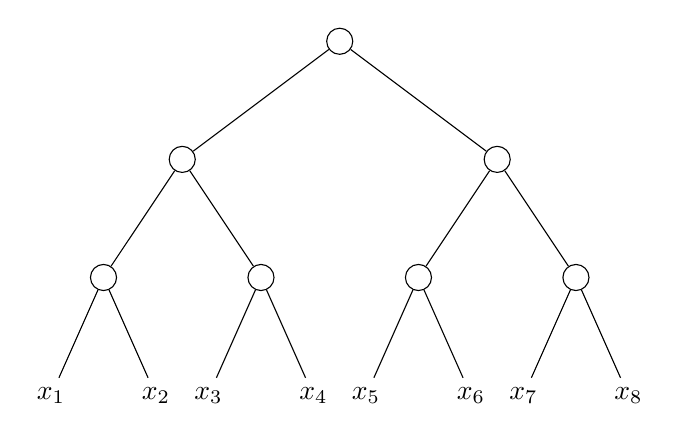
\begin{tikzpicture}[level/.style={sibling distance=40mm/#1}]
	\node [circle,draw]    (z){}
	
	child {node [circle,draw]    (a) {}
		child {node [circle,draw]    (b) {}
			child {node {$x_1$}}
			child {node {$x_2$}}
		}
		child {node [circle,draw]    (g) {}
			child {node {$x_3$}}
			child {node {$x_4$}}
		}
	}
	child {node [circle,draw]    (j) {}
		child {node [circle,draw]    (k) {}
			child {node {$x_5$}}
			child {node {$x_6$}}
		}
		child {node [circle,draw]    (l) {}
			child {node {$x_7$}}
			child {node {$x_8$}}
		}
	};
	\end{tikzpicture}%}
\end{figure}


Luego, la estructura de árbol resulta natural al momento de representar los números $p$-ádicos tomando $C=\frac{1}{p}$ para $\gpn$. Luego, la implementación de un modelo para el conjunto $\mathit{G2\_22}\subset \Q_2$ (con $p=2$, $n=-2$ y $N=1$), está dado por:
\label{list_repreTree}
\begin{lstlisting}[language = Python, caption = Representación en árbol de $\mathit{G2\_21}$]
G2_21 = GpnN   (2,-2,1) #initialization
G2_21.generate_numbers()
G2_21.representation_tree()
\end{lstlisting}

\newpage
\newpage
Así, la función \texttt{representation\_tree()} mostrada en el anterior código, exportará una imagen en formato PNG de la siguiente forma:
\begin{center}	
	\includegraphics[scale=0.8]{img/G2_21}
\end{center}
Donde los nodos hoja representan números de la forma: $$x=\sum_{-1}^{2}a_k2^k = a_{-1}\cdot2^{-1}+a_0\cdot 2^0 + a_1\cdot 2 + a_2\cdot 2^2,$$

y que además satisfacen $2^{-2}\leq\norm{x}_2\leq 2$. Dado que los $a_k\in\{0,1\}$, con $k\in\{-1,0,1,2\}$, denotamos la elección de $a_k$ por las aristas del árbol, así, decir que $a_k\in\{\textbf{0},\textbf{\textcolor{red}{1}}\}$ será equivalente a decir que $a_k\in\{\textbf{Negro},\textbf{\textcolor{red}{Rojo}}\}$
en este ejemplo. 

Luego, si quisiéramos saber qué número es el que está ubicado en la parte derecha del árbol, de color \textbf{\textcolor{blue}{azul}}, sólo seguimos el camino propuesto por la imagen. Así, partiendo desde la raíz, tenemos que el camino hasta llegar a este nodo será $\textbf{Negro}\to\textbf{Negro}\to\textbf{Negro}\to\textbf{\textcolor{red}{Rojo}},$ es decir que el número es \textbf{000,}\textbf{\textcolor{red}{1}}$_2$ y tiene norma \textbf{\textcolor{blue}{$2^{-1}$}}; tal como lo indica la barra ubicada en la parte derecha de la imagen. Nótese que el camino desde la raíz denota $a_2\to a_1\to a_0\to a_{-1}$.
\begin{remark}
	En casos más generales, el entendimiento de la imagen será parecido. Luego, entre más grande sea el primo, más colores en las aristas habrá, así como habrá más normas y el recorrido de los elementos desde la raíz denotará $a_{-n}\to a_{n-1}\to\cdots\to a_0 \to \cdots \to a_{-N+1} \to a_{-N}.$
\end{remark}
\begin{figure}
	\begin{subfigure}{.5\textwidth}
		\centering
		\includegraphics[width=.8\linewidth]{img/G2_22}
		\caption{$\mathit{G2\_22}$}
		\label{fig:sfig1}
	\end{subfigure}%
	\begin{subfigure}{.5\textwidth}
		\centering
		\includegraphics[width=.8\linewidth]{img/G2_32}
		\caption{$\mathit{G2\_32}$}
		\label{fig:sfig2}
	\end{subfigure}
	\begin{subfigure}{.5\textwidth}
		\centering
		\includegraphics[width=.8\linewidth]{img/G2_33}
		\caption{$\mathit{G2\_33}$}
		\label{fig:sfig1}
	\end{subfigure}%
	\begin{subfigure}{.5\textwidth}
		\centering
		\includegraphics[width=.8\linewidth]{img/G2_43}
		\caption{$\mathit{G2\_43}$}
		\label{fig:sfig1}
	\end{subfigure}%
	\caption{Representación en árbol de los números $2$-ádicos.}
	\label{2adics_trees}
\end{figure}